\documentclass[UTF8]{ctexart}
\usepackage{geometry}
\geometry{a4paper, margin=2.5cm}
\usepackage{graphicx}
\usepackage{listings}
\usepackage{xcolor}
\usepackage{float}
\usepackage{hyperref}
\usepackage{url}
\hypersetup{colorlinks=true, linkcolor=blue, urlcolor=blue}
\graphicspath{{D:/code/LATEX/ComputerNetworkingReport}}

\lstset{
    basicstyle=\ttfamily\small,
    keywordstyle=\color{blue},
    commentstyle=\color{gray},
    stringstyle=\color{red},
    breaklines=true,
    frame=single,
    numbers=left,
    numberstyle=\tiny,
    tabsize=2,
}

\title{\textbf{DASH实验报告：BBA-0算法实现与分析}}
\author{严子竣}
\date{\today}

\begin{document}

\maketitle

\section{搭建流程}

1.获取dash.js，安装node.js和npm并配置环境变量等流程，与所提供的文档一致，此处不再赘述。

2.使用虚拟机（Ubuntu 22.04）配置服务器：安装server版，搭建结果如图\ref{fig:virtualmachine}和图\ref{fig:port}所示：

\begin{figure}[H]
    \centering
    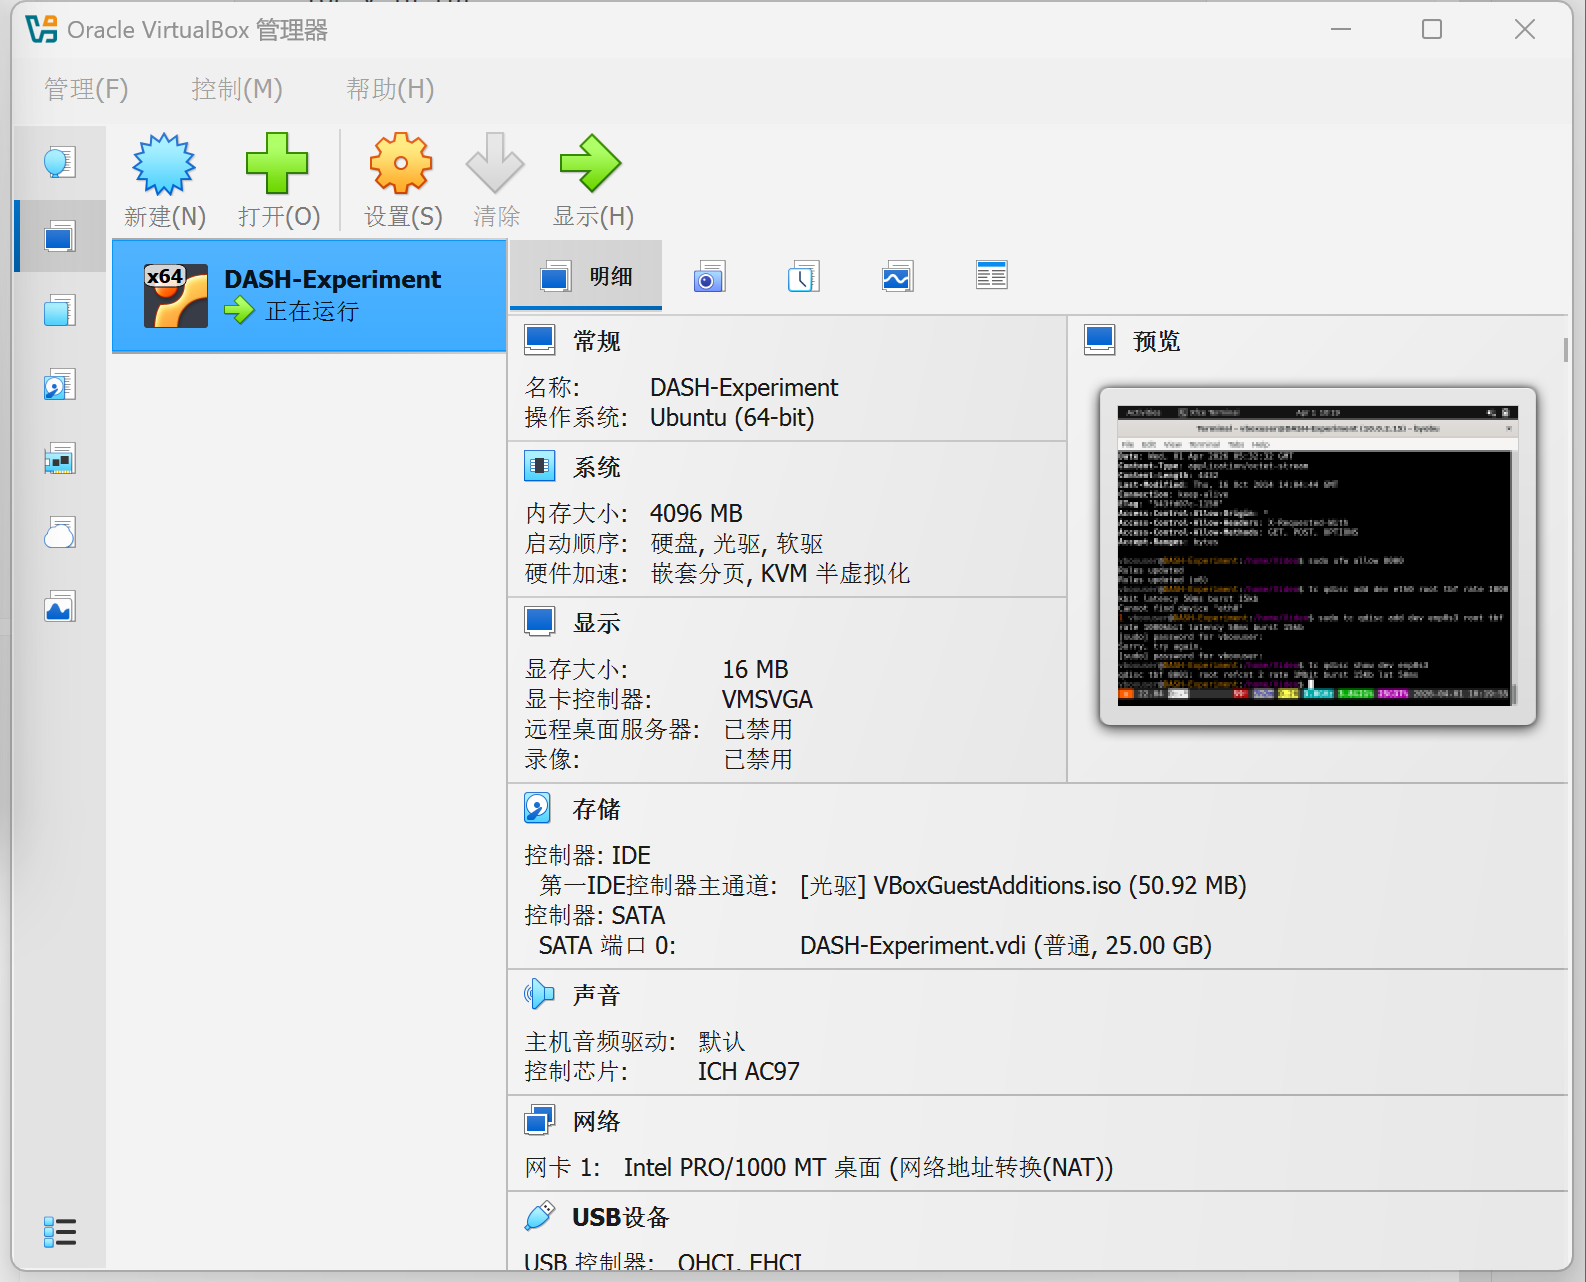
\includegraphics[width=0.7\textwidth]{virtualmachine.png}
    \caption{虚拟机}
    \label{fig:virtualmachine}
\end{figure}
\begin{figure}[H]
    \centering
    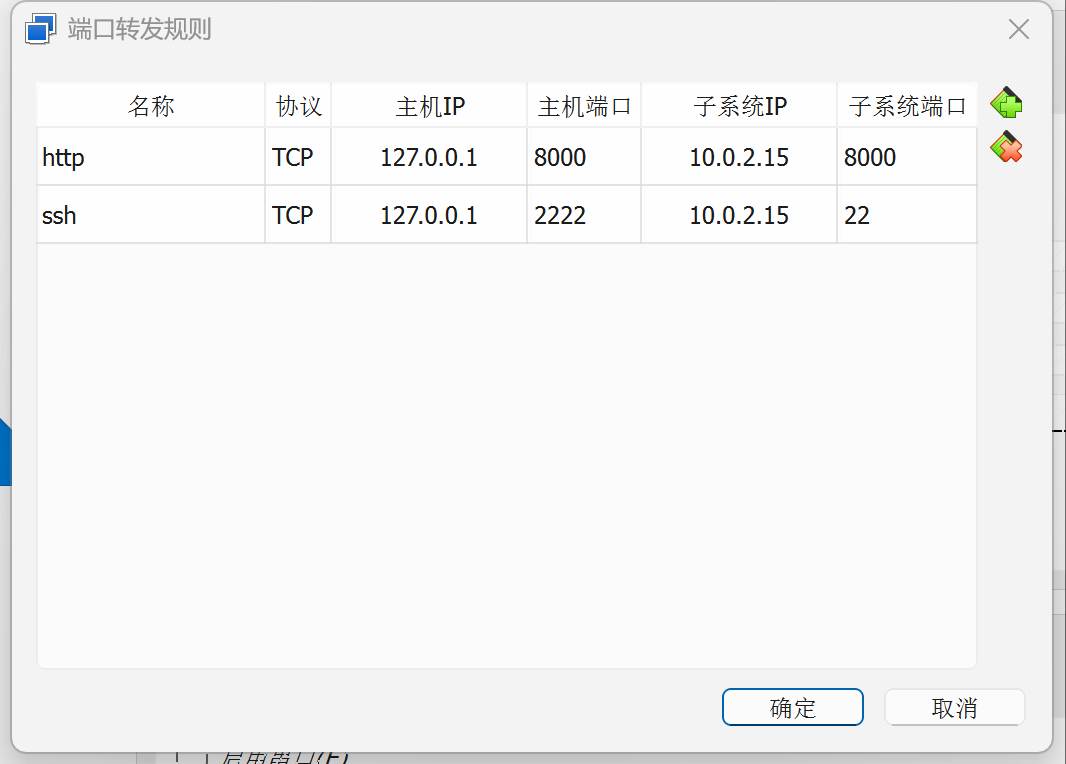
\includegraphics[width=0.7\textwidth]{port.png}
    \caption{端口转发规则}
    \label{fig:port}
\end{figure}

3.安装nginx

\begin{figure}[H]
    \centering
    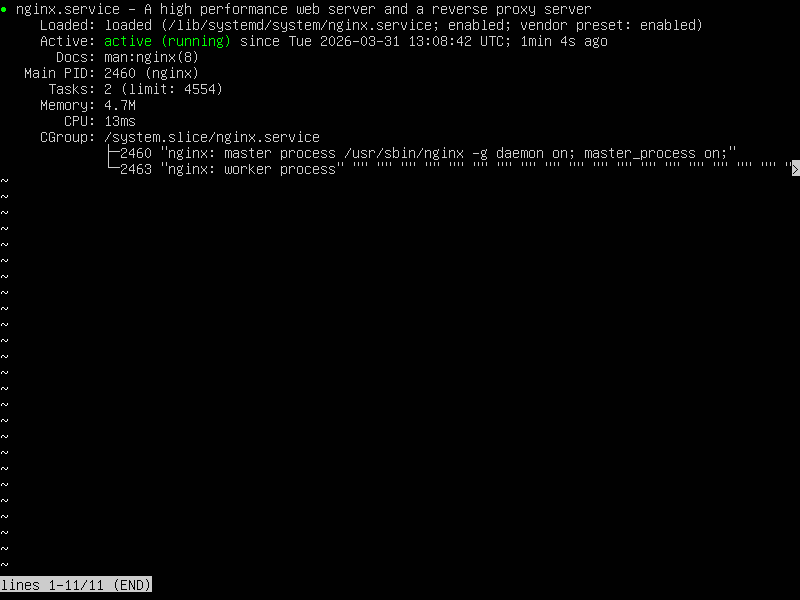
\includegraphics[width=0.7\textwidth]{nginx.png}
    \caption{nginx安装结果}
    \label{fig:nginx}
\end{figure}

安装nginx后，修改Nginx配置文件 \texttt{/etc/nginx/nginx.conf}，添加如下server块：

\begin{lstlisting}
server {
    listen 0.0.0.0:8000;
    server_name 127.0.0.1;
    add_header Access-Control-Allow-Origin *;
    add_header Access-Control-Allow-Headers X-Requested-With;
    add_header Access-Control-Allow-Methods GET,POST,OPTIONS;
    location / {
        root /home/video;
        autoindex on;
    }
}
\end{lstlisting}
重启Nginx：\texttt{sudo systemctl restart nginx}。  \\
通过浏览器访问 \texttt{http://10.0.2.15:8000/} 能看到视频文件列表，证明服务器配置成功。

4.获取视频文件：进入目录/home/Video，使用wget递归下载2sec版本的视频文件：
\begin{lstlisting}[language=bash]
    cd /home/Video
    wget -r -np -nH --cut-dirs=4 -R "index.html*" http://ftp.itec.aau.at/datasets/DASHDataset2014/BigBuckBunny/2sec/
\end{lstlisting}

再使用scp将视频上传至服务器（未及时保存截图，找不到了）。

在dash.js中输入：\\
 \texttt{http://127.0.0.1:8000/BigBuckBunny/2sec/BigBuckBunny\_2s\_simple\_2014\_05\_09.mpd}\\
  能够正常播放，说明上传成功。

5.使用tc限制服务器的网络带宽

\begin{lstlisting}[language=bash]
    sudo tc qdisc add dev enp0s3 root tbf rate 1000kbit latency 50ms burst 15kb
\end{lstlisting}

\begin{figure}[H]
    \centering
    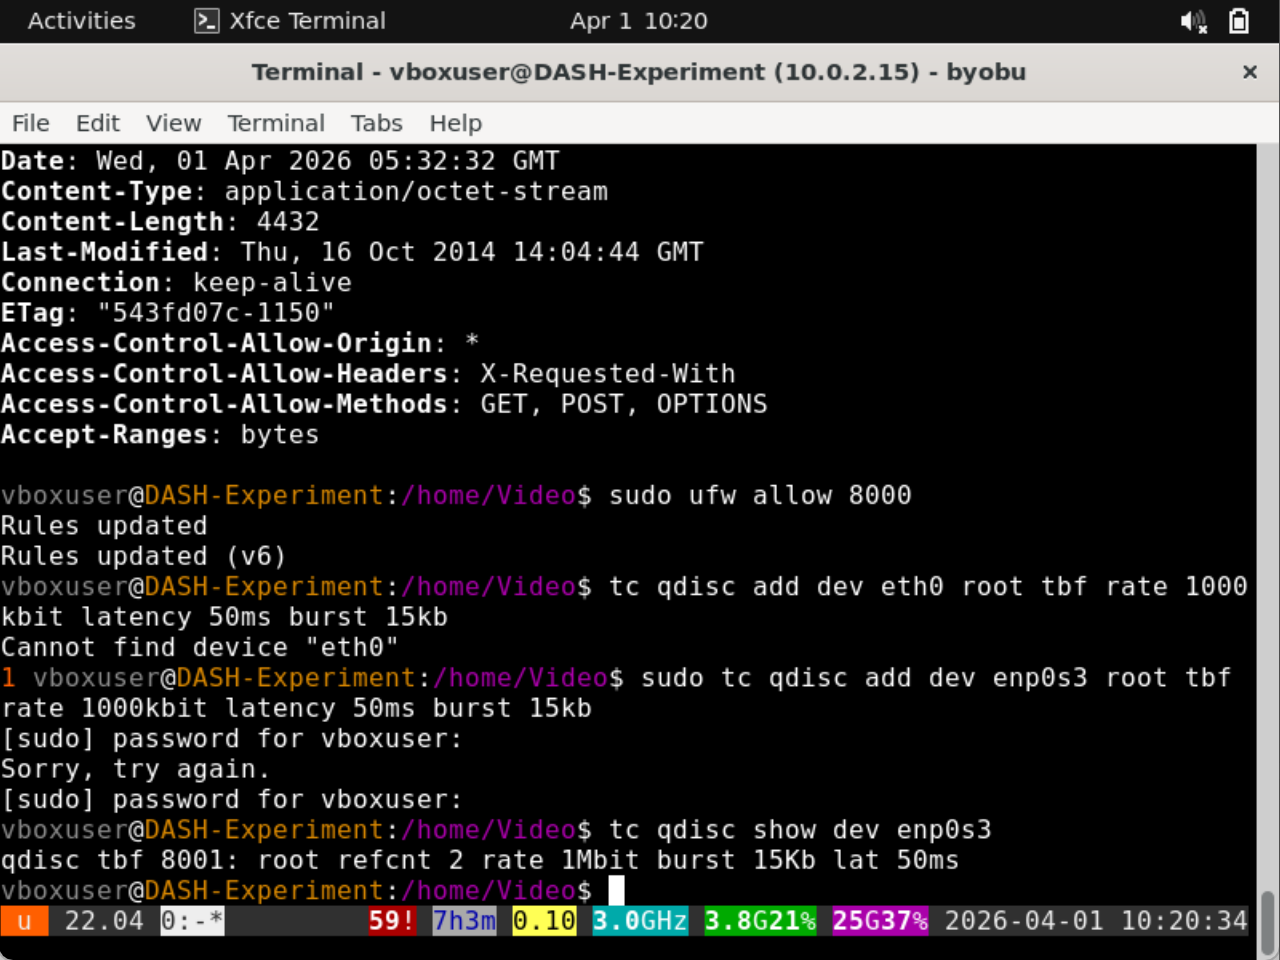
\includegraphics[width=0.7\textwidth]{tc.png}
    \caption{使用tc限制带宽}
    \label{fig:tc}
\end{figure}

\section{实现的ABR算法：BBA-0}
BBA-0完全基于缓冲区长度（秒）决策码率，定义低阈值$L=10$秒、高阈值$H=30$秒：
\begin{itemize}
    \item 缓冲区 $< L$：选择最低码率。
    \item 缓冲区 $> H$：选择最高码率。
    \item 缓冲区在 $[L, H]$：线性插值 $$\mathrm{index} = \left\lfloor \frac{B-L}{H-L} \times (N-1) \right\rfloor$$
    其中$N$为码率等级数。
\end{itemize}
在dash.js中新建\texttt{BBARule.js}，实现\texttt{getMaxIndex}方法，注册到\texttt{AbrController}，并在HTML界面添加“BBA-0”选项。

代码如下：

\begin{lstlisting}[language=Java, caption=BBARule.js]
import FactoryMaker from '../../../core/FactoryMaker.js';

function BBARule() {
    const lowThreshold = 10;
    const highThreshold = 30;

    const instance = {
        getMaxIndex: function (rulesContext) {
            const abrController = rulesContext.getAbrController();
            const mediaInfo = rulesContext.getMediaInfo();
            const bufferLevel = rulesContext.getBufferState().getBufferLevel();
            const bitrateList = abrController.getBitrateList(mediaInfo);

            if (!bitrateList || bitrateList.length === 0) return -1;
            if (bufferLevel === undefined) return bitrateList.length - 1;

            let targetBitrateIndex;

            if (bufferLevel <= lowThreshold) {
                targetBitrateIndex = 0; // 最低码率
            } else if (bufferLevel >= highThreshold) {
                targetBitrateIndex = bitrateList.length - 1; // 最高码率
            } else {
                // 线性插值
                const ratio = (bufferLevel - lowThreshold) / (highThreshold - lowThreshold);
                const maxIndex = bitrateList.length - 1;
                targetBitrateIndex = Math.floor(ratio * maxIndex);
            }

            // 保证索引有效
            targetBitrateIndex = Math.min(Math.max(targetBitrateIndex, 0), bitrateList.length - 1);
            return targetBitrateIndex;
        }
    };

    return instance;
}

BBARule.__dashjs_factory_name = 'BBARule';
export default FactoryMaker.getClassFactory(BBARule);

\end{lstlisting}

\section{生效结果与分析}
使用tc限制带宽为2Mbps，播放时观察客户端下方监控图（图\ref{fig:monitor}）。当缓冲区低于10秒时，码率立即降为最低档（约0.5 Mbps）；缓冲区上升至10–30秒区间时，码率随缓冲区线性增加；超过30秒后稳定在最高码率。带宽恢复后，缓冲区重新积累，码率平缓回升。整个过程无卡顿，验证了BBA-0的鲁棒性。

\begin{figure}[H]
    \centering
    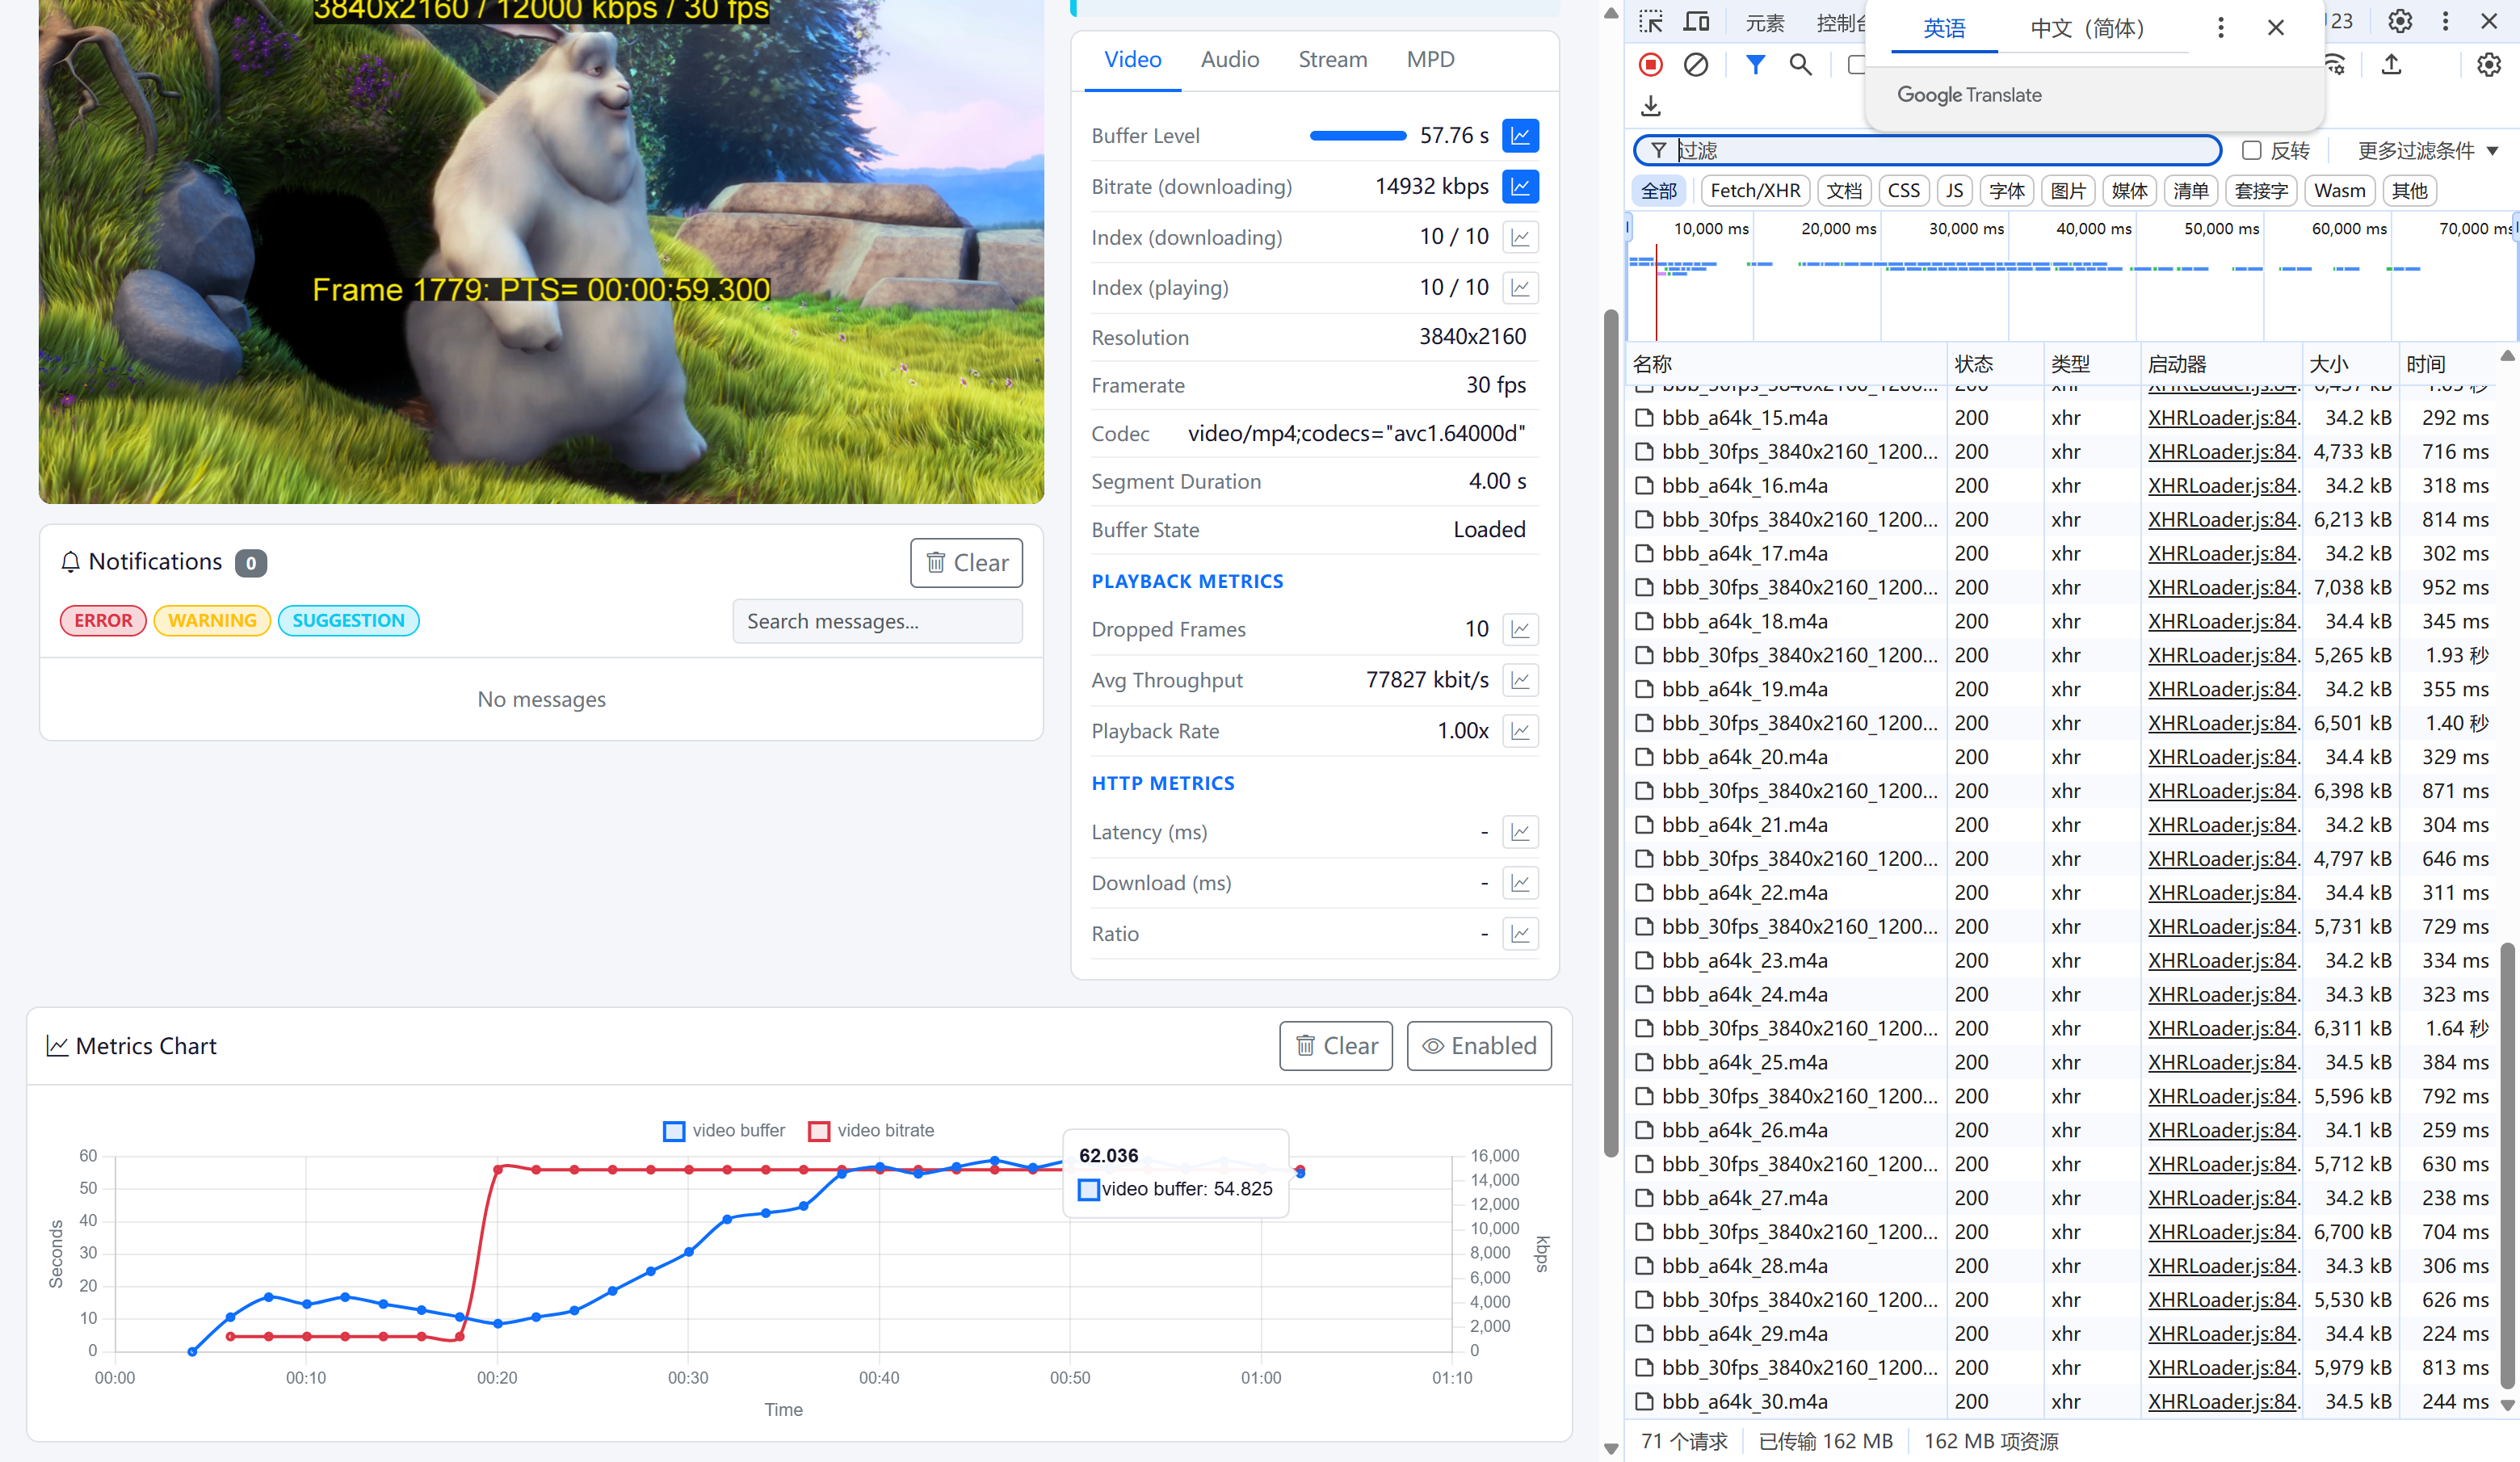
\includegraphics[width=\textwidth]{monitor.png}
    \caption{客户端码率与缓冲区监控图}
    \label{fig:monitor}
\end{figure}

\section{学习总结}
\begin{itemize}
    \item \textbf{DASH}：将视频切分为分片并提供MPD描述文件，客户端自主请求合适码率的分片，实现了服务器与客户端的解耦。
    \item \textbf{BBA}：仅根据当前缓冲区占用量（buffer occupancy）来决定请求的码率，完全不依赖网络吞吐量预测，从而避免吞吐量预测不准带来的问题。
\end{itemize}

\end{document}